\section{Software para operaciones de conjuntos}

He escrito este sencillo software como parte de los proyectos para la materia de Matemáticas Discretas.\\

Dicho software está escrito en C\# .Net, tanto el CORE como la GUI.\\

He elegido este lenguaje de programación debido a la sencillez relativa para crear la interfaz del usuario y a la fluidez propia de .Net para escribir código que funcione ``Out of the Box'' (para Windows, claro).\\

Las operaciones que este software realiza son las siguientes:\\
* Union\\
* Intersección\\
* Diferencia\\
* Producto Cartesiano\\

La única pantalla que posee el software es la que se muestra en la Fig~\ref{img:1}.\\


\begin{figure}[h]
\centering
    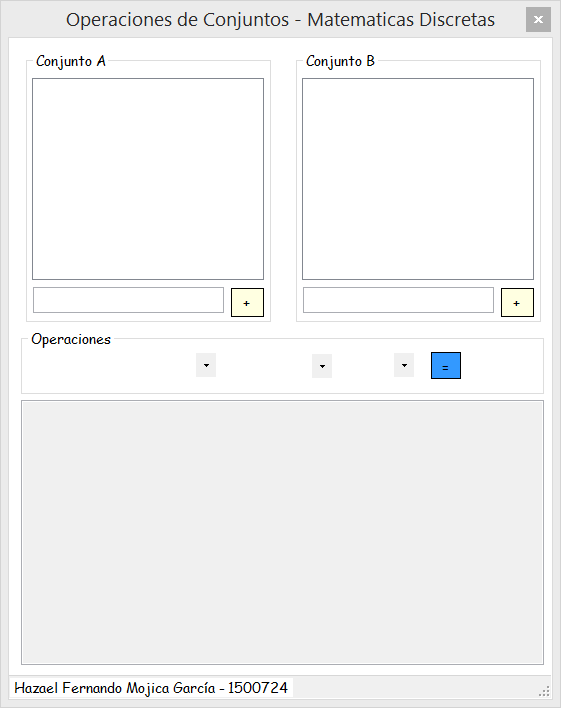
\includegraphics[angle = 0]{img/1.png}
    \caption{GUI de la aplicación}
	\label{img:1}
\end{figure}

\subsection{Funcionamiento}

Los pasos a seguir para poder realizar operaciones usando esta aplicación son los siguientes:\\

1.- Introducir un conjunto de elementos en el campo del Conjunto A tal y como se muestra en la Fig~\ref{img:2} tecleando el valor del elemento y dando Enter para insertarlo o presionando el botón \textbf{+}. Hacer lo mismo con el Conjunto B.\\

2.- Una vez se tengan los dos conjuntos listos seleccionar el tipo de operación y los conjuntos a los cuales aplicar dicha operación (A con B, A con A, B con B, B con A), ver Fig~\ref{img:3},se quiso dejar de esta manera para poder ampliar esta aplicación a un número N de conjuntos si era necesario en el futuro.\\

3.- Presionar el botón \textbf{=} y ver el resultado en el cuadro de texto inferior. Todos los resultados incluyen el conjunto vacío. Fig~\ref{img:4}.\\

* Es posible eliminar elementos de cada conjunto seleccionando el elemento y presionando la tecla \textbf{Del / Supr}

\begin{figure}[h]
\centering
    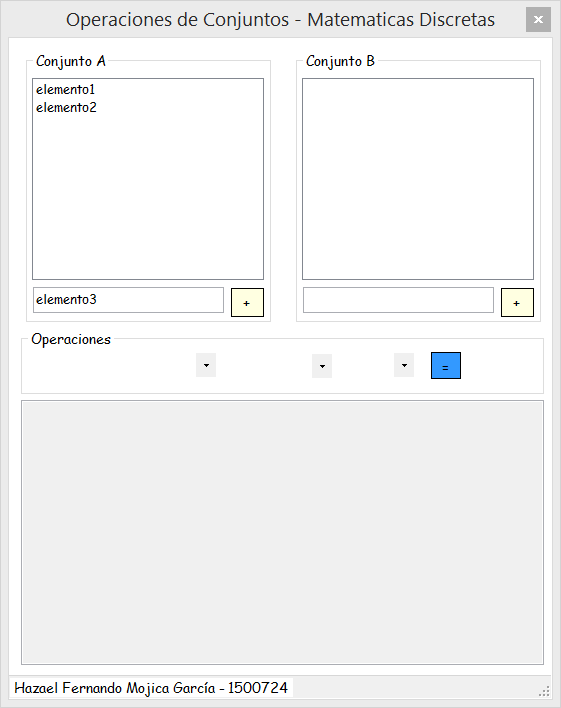
\includegraphics[angle = 0]{img/2.png}
    \caption{Introducir los elementos de ambos conjuntos}
	\label{img:2}
\end{figure}

\begin{figure}[h]
\centering
    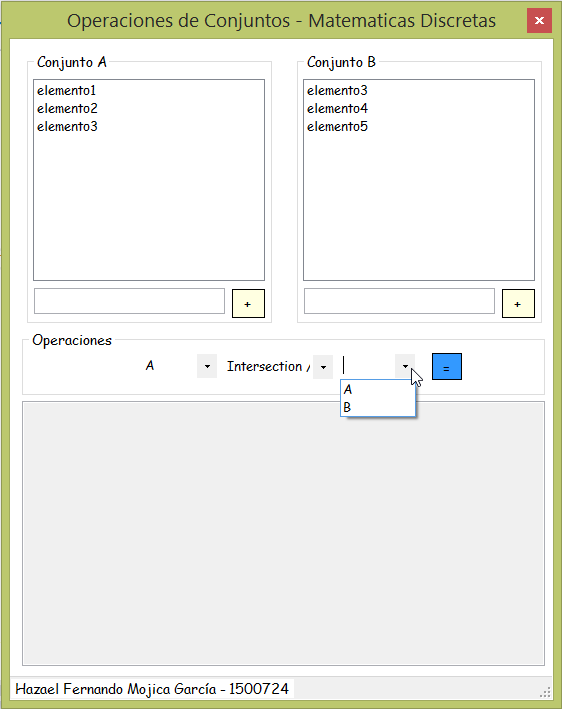
\includegraphics[angle = 0]{img/3.png}
    \caption{Seleccionar los conjuntos y las operaciones a realizar con ellos}
	\label{img:3}
\end{figure}

\begin{figure}[h]
\centering
    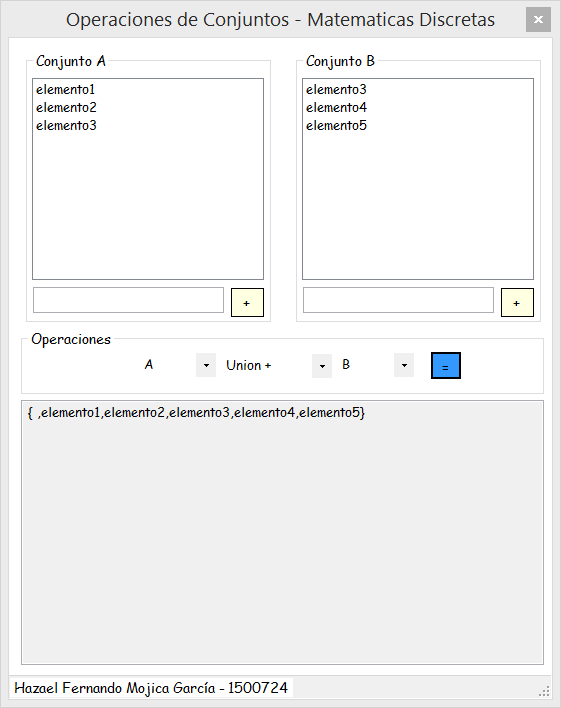
\includegraphics[angle = 0]{img/4.png}
    \caption{Resultado}
	\label{img:4}
\end{figure}

\newpage

\subsection{Código}

Colocaré aquí únicamente la \textbf{clase Set}, el demás código escrito se encarga de la creación de la GUI y de su interacción con el usuario.\\

La clase Set se encarga completamente del almacenamiento del conjunto, y del  cálculo y operaciones con los mismos.\\

Los elementos del conjunto se guardan como una instancia de la clase List<string>, se hace incapie a que esta estructura permite agregar y eliminar elementos de manera sencilla y con alto rendimiento además que permite el uso de datos genéricos y s fuertemente tipada.\\

He creado dos constructores, uno vacío y otro donde se pasa el conjunto.\\

Los métodos creados son descriptivos por sí mismos, solo hace falta una ojeada rápida a los mismos para entender su funcionamiento.


\begin{lstlisting}
/**
 Author: Hazael Fernando Mojica Garcia.
 */

using System;
using System.Collections;
using System.Collections.Generic;
using System.Linq;
using System.Text;
using System.Threading.Tasks;

namespace conjuntos
{
    class Set
    {
        private List<string> items;

        /*CONSTRUCTORS*/
        /*************************************************************************************************/

        public Set()
        {
            //Add Empty Item
            initEmpty();
        }

        /// <summary>
        /// Class Constructor
        /// </summary>
        /// <param name="items">A string array which represent the items</param>
        public Set(List<string> items)
        {
            if (items != null)
                this.items = items;
            else
                initEmpty();
        }

        private void initEmpty()
        {
            this.items = new List<string>();
            this.items.Add(" ");
        }
        /*END CONSTRUCTORS*/
        /*************************************************************************************************/

        public List<string> getItems()
        {
            return this.items;
        }


        /// <summary>
        /// Applies the Intersection operation to this Set
        /// </summary>
        /// <param name="set_">The set to apply Intersection operation to this one</param>
        /// <returns>An instance os Set with the result of the Intersection operation</returns>
        public Set intersection(Set set_)
        {
            Set resultSet;
            List<string> setArray_ = set_.getItems();
            List<string> resultArray = new List<string>();

            for (int i = 0; i < setArray_.Count; i++)
            {
                if (this.items.Contains(setArray_[i]))
                    resultArray.Add(setArray_[i]);
            }
            resultSet = new Set(resultArray);
            return resultSet;
        }

        /// <summary>
        /// Applis the Union operation to this Set
        /// </summary>
        /// <param name="set_">The set to apply the Union operation to this one</param>
        /// <returns>An instance os Set with the result of the Union operation</returns>
        public Set union(Set set_)
        {
            Set resultSet;
            List<string> setArray_ = set_.getItems();
            List<string> resultArray = new List<string>(this.items);

            for (int i = 0; i < setArray_.Count; i++)
            {
                if(!resultArray.Contains(setArray_[i]))
                    resultArray.Add(setArray_[i]);
            }
            resultSet = new Set(resultArray);
            return resultSet;
        }

        /// <summary>
        /// Applis the difference operation to this Set (this.set - set_)
        /// </summary>
        /// <param name="set_">The set to apply the difference operation to this one</param>
        /// <returns>An instance os Set with the result of the difference operation</returns>
        public Set difference(Set set_)
        {
            Set resultSet;
            List<string> setArray_ = set_.getItems();
            List<string> resultArray = new List<string>(this.items);

            for (int i = 0; i < setArray_.Count; i++)
            {
                if (resultArray.Contains(setArray_[i]))
                    resultArray.Remove(setArray_[i]);
            }

            //Insert empty item (it has been eliminated)
            resultArray.Insert(0, " ");
            resultSet = new Set(resultArray);
            return resultSet;
        }

        /// <summary>
        /// Apply the cartesian operation to this Set
        /// </summary>
        /// <param name="set_">The set to apply the Union operation to this one</param>
        /// <returns>An instance os Set with the result of the cartesian Product operation</returns>
        public Set cartesianProduct(Set set_)
        {
            Set resultSet;
            List<string> setArray = new List<string>(this.items);
            List<string> setArray_ = set_.getItems();
            List<string> resultArray = new List<string>();

            //Remove both empty items
            setArray.RemoveAt(0);
            setArray_.RemoveAt(0);

            for (int i = 0; i < setArray.Count; i++)
            {
                for (int j = 0; j < setArray_.Count; j++)
                    resultArray.Add("(" + setArray[i] + ", " + setArray_[j] + ")");
            }

            //Add empty item
            resultArray.Insert(0, " ");
            resultSet = new Set(resultArray);
            return resultSet;
        }

        public override string ToString()
        {
            string itemsS = "";
            itemsS += "{";
            for (int i = 0; i < this.items.Count; i++)
                itemsS += this.items[i].ToString() + ",";
            //Delete last comma
            itemsS = itemsS.Substring(0, itemsS.Length - 1);
            itemsS += "}";

            return itemsS;
        }
    }
}

\end{lstlisting}